%Sección
\section{Ciencia de Datos}
\lhead[\thepage]{\thesection Ciencia de Datos}

\subsection{Definición}

La Ciencia de Datos es el estudio del origen de la información, que representa  y como puede convertirse en un recurso valioso en los planes estratégicos de las organizaciones.\cite{1rouse}

Se considera una etapa evolutiva, dada por la unión de varios campos interdisciplinarios como la inteligencia de negocios, el modelado estadístico y las matemáticas.\cite{2whatisdatasc}Tambien comprende área tales como: minería de texto, computación paralela y distribuida, \emph{machine learning}, bases de datos NoSQL, herramientas para visualización, entre otras.

En la actualidad se enfoca fuertemente en el área de \emph{Big Data} donde es necesario el trabajo conjunto de diversas áreas para poder llevar a cabo procesos de análisis, para trabajar con cantidades masivas de datos.

\subsection{Rol del Científico de Datos}

El científico de datos, es aquel que obtiene conocimiento a partir de un conjunto de datos para responder a preguntas que se le han formulado.\cite{5pellicer} Generalmente posee gran experiencia y un alto grado de conocimiento en una de las áreas interdisciplinarias de la ciencia de datos y un conocimiento avanzado en algunas de las otras que conforman esta disciplina. 

Es considerado como un nuevo perfil profesional, evolución del analista de negocio o analista de datos \cite{3carbo,4uespana,5pellicer}. Aunque su enfoque sobrepasa al de la inteligencia de negocios, se adentra en la exploración y análisis de datos de múltiples fuentes y formatos, buscando las soluciones de mayor valor para la organización \cite{5pellicer}.
 El papel del científico de datos es variado, en el mercado laboral de la industria de ciencia de datos surgen distintos roles dependientes de aspectos como, las herramientas o tecnologías que deben manejarse en el área, habilidades o técnicas  utilizadas al abordar un problema. Para poder manejar estos aspectos un cientifico de datos debe tener una formación solida en ciencias de la computación y aplicaciones, modelado, estadísticas, análisis y matemáticas \cite{5pellicer}.

 \begin{figure}[!htbp]
    \centering
    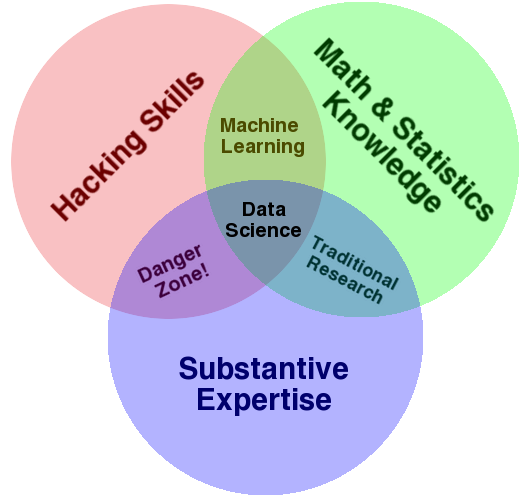
\includegraphics[width=0.7\textwidth]{Figuras/Data_Science_VD.png}
    \caption{Diagrama de Ven, habilidades del científico de datos}
    \label{fig:vennskills}
    \source{http://drewconway.com/zia/2013/3/26/the-data-science-venn-diagram}
\end{figure}

 Debido a la variedad de roles que debe cumplir un científico de datos, el trabajo en ciencia de datos no es realizado por un único individuo. La tendencia es crear equipos multidisciplinarios donde aquellos que los componen (científicos de datos) ocupan distintos roles con una especialidad y función en concreto (como se ejemplifica en la Figura \ref{fig:vennskills}), pero con nociones esenciales de las funciones de los otros miembros del equipo \cite{5pellicer}.

\subsection{Grandes Volúmenes de Datos (\emph{Big Data})}

\subsubsection{Definición}

EL termino grandes volúmenes de datos (conocido en el ámbito comercial como \emph{Big Data}), se refiere a cantidades masivas de datos (tanto estructurados, no estructurados y semi-estructurados), que superan la capacidad de las bases de datos relacionales convencionales para poder ser almacenados, administrados y procesados en un tiempo  aceptable \cite{7sasinc}.

El crecimiento contante de los volúmenes de datos requiere de tecnologías rentables, y eficientes en el manejo del tiempo, que puedan ser usadas para generar conocimiento de valor para la toma de decisiones \cite{8gartner,9ibm}.

 
El ``Modelo de las 3 V's" de Doug Laney \cite{10laney}, recoge las definiciones de tres aspectos fundamentales de los datos, que para el 2001 eran manejados en el área de \emph{E-commerce} o comercio electrónico, sin embargo el modelo planteado por Laney sirvió de punto de apoyo en los inicios de \emph{Big Data}. Estos atributos claves son : volumen, velocidad y variedad.

\begin{itemize}
\item Volumen:  se refiere a la vasta cantidad de datos que se generan cada segundo. Estos volúmenes de datos que aumentan constantemente, hacen que su almacenamiento y análisis imposible usando tecnologías tradicionales de base de datos. La tecnología usada en el área de Big Data se enfoca en solucionar este problema utilizando sistemas distribuidos, donde partes de los datos son almacenados en diferentes locaciones, conectadas a  través de redes y utilizadas como un solo sistema \cite{13bernard}.

\item Velocidad: hace referencia a la velocidad a la que se generan, transmiten, procesan y almacenan nuevos datos. El incremento de este atributos en el ámbito de la generación y transmisión de datos a contribuido con la existencia de Big Data, mientras que el aumento en la velocidad de procesamiento, almacenamiento y también transmisión han sido esenciales para su análisis, lo que ha permito dar respuestas de forma más rápida a las necesidades especificas de cada negocio\cite{11pragsis}. 

  \begin{itemize}
  \item Viscocidad: atributo asociado con el retardo o latencia del tiempo de alguno de los eventos asociados a la velocidad \cite{16}. 
  \item Viralidad: atributo que describe la velocidad con la que los datos se propagan, la frecuencia con la que son recuperados y repetidos entre usuarios o eventos \cite{16}.
  \end{itemize}
 \item Variedad: se refiere a los diferentes tipos de datos que sirven de fuente, estos datos pueden venir de archivos de texto plano, correos electrónicos, fotos, vídeos, logs de transacciones, redes sociales, paginas web, entre otros \cite{13bernard}. Esta variedad no solo aplica al medio de donde proviene también a su tipo de estructura (estructurados, semi estructurados, no-estructurados). 
 
\end{itemize}

Existen nuevos modelos que surgen de la evaluación del área de \emph{Big Data} y su constante evolución, acontinuacion se definen estas nuevas variables que se incorporan a \emph{Big Data}:

 \begin{itemize}
 \item Valor: este atributo busca ponderar la utilidad de la información que puede ser obtenida de los datos. Un error común y fácil de cometes es la toma de iniciativas de grandes volúmenes de datos sin una clara comprensión del valor de negocio que traerá, esta variable es de gran importancia para medir si vale la pena comenzar un proceso de análisis de \emph{Big Data}. Ciertos autores afirman que ésta variable no depende de si se trabaja con grandes volúmenes de datos o no, puesto a que es un indicador clave en cualquier proceso de análisis \cite{16}.
 
\item Veracidad: nivel de certidumbre de los datos. Debido a la variedad de los datos, la calidad y precisión de los mismos es más difícil de controlar. Los volúmenes a menudo compensan la falta de calidad o exactitud, a partir de la cual cobra importancia la variable del valor \cite{13bernard}. La tarea de verificar la veracidad de los datos es compleja, es necesario evaluar el contexto de los datos teniendo en cuenta su procedencia, la comprensión de los mismos es importante para su utilización \cite
{18}. El científicos de datos emplean hasta un 80\% de su tiempo, en la limpieza y pre-procesamiento de los datos para asegurar un indice alto de veracidad.

\item Variabilidad: hace referencia a los cambios constante en los datos. La naturaleza de los datos no siempre es estáticas y su significado podría variar mucho en su contexto \cite{15}.

\item Visualización: atributo asociado a la representacion dada de forma visual a los datos ya procesados para su fácil entendimiento. La visualización de grandes volúmenes de datos pueden contener decenas de variables y parámetros, lo que resulta en un reto para \emph{Big Data} el como presentar estos \cite{15}. La visualización es fundamental al ser esta la manera en como se harán accesibles los datos procesados para las organizaciones. Otro aspecto a tomar en cuenta de la visualización es cuando esta variable forma parte del proceso de análisis a través de la exploración visual de datos, que puede servir como herramienta al científico de datos, la visualización de datos ayudará a los científicos a comprender qué técnicas podrían ser mejor utilizados para descubrir ideas o patrones ocultos y les ayudará a entender los resultados de la aplicación de estas técnicas, lo que ayuda a guiar el proceso de análisis de los resultados deseados \cite{17}.

\item Validez: la validez de los datos es esencial para la toma de decisiones, debido a que usar datos de fuentes  no confiables puede llevar el proceso de análisis por una ruta errónea. Los datos de entrada válidos, seguido por el procesamiento correcto de los mismos, deben dar resultados exactos.

\item Volatilidad: se refiere al tiempo en el cual los datos son válidos y por cuanto tiempo deben almacenarse, debido al factor de la variabilidad la utilidad de los datos puede cambiar, será necesario determinar en qué momento dichos datos ya no serán relevantes para el análisis actual \cite{14}.

\item Vialidad: es descrita como una cuidadosa selección de los atributos en los datos que tienen más probabilidades de predecir los resultados de mayor importancia para las organizaciones \cite{18}. Mientras que se considera que tan solo el 5\% de los atributos en los datos son responsables del 95\% de los beneficios, por lo que se debe de considerar esta cualidad\cite{19}, otros autores consideran que la vialidad no es una propiedad propia de \emph{Big Data}, sino que es una cualidad que se determina mediante el análisis de los grandes volúmenes de datos  \cite{18}.

 \end{itemize}
 
 
% \subsection{Campos Donde es Utilizado}

% 	Las posibilidades de la Ciencia de Datos y \emph{Big Data} son inmensas, existen una gran cantidad sectores que se benefician de este nuevo paradigma, afecta a las organizaciones de prácticamente cualquier industria \cite{7sasinc}:

% \begin{itemize}
% \item Ciencias Sociales: Redes sociales como Facebook o Twitter, generan millones de datos diariamente \cite{https://www.gwava.com/blog/internet-data-created-daily}, dicha data es ahora aprovechable gracias a la capacidad y enfoque que tienen las herramientas y tecnologias que han surgido para el manejo de \emph{Big Data}.

% \item Ciencias Económicas: sistemas de recomendaciones implementados por Amazon o Netflix son claros ejemplos de cómo los grandes volúmenes de datos han sido aprovechados para ayudar a entender y servir mejor a los clientes.

% \item Medicina: las agencias gubernamentales pueden ahora predecir brotes de enfermedades y hacer seguimientos en tiempo real, para que las compañías farmacéuticas puedan acelerar el desarrollo de los fármacos necesarios. Recientemente Google estudiaba implementar un algoritmo para predecir la propagación del Zika en el mundo y poder ayudar a destinar ayudas humanitarias por parte de los Gobiernos [21].

% \item Gobierno: las agencias gubernamentales son capaces de aprovechar los grandes volúmenes de datos para ayudar a los servicios públicos a afrontar mejor sus retos, frente a congestiones de tráfico, prevención de la delincuencia. frustrar ataques terroristas, detectar delitos cibernéticos, entre otros. Otras entidades como la Organización de las Naciones Unidas han destinado presupuestos para el financiamiento de proyectos de ayuda humanitaria y tratamiento del medio ambiente, como es el caso del Pulso Global.

% \item Deportes: distintos dispositivos y sensores que permiten el análisis de datos en tiempo real por medio del Internet de las Cosas, ha permitido mejorar el rendimiento de los deportistas, siendo equipos como el Real Madrid, la selección oficial de fútbol Alemana en el Mundial de Brasil 2014, escuderías de la fórmula uno como la McLaren, entre otros participantes de éste tipo de avances.

% \item Educación: el análisis de los grandes volúmenes de datos permite a los educadores tener una visión del progreso de los estudiantes, pudiendo implementar sistemas para la evaluación y mejora en el rendimiento de los mismos.

% \end{itemize}


% La ciencia de datos ofrece por tanto, nuevos y potentes enfoques para hacer descubrimientos, mediante la combinación de los campos de la estadística, computación y matemáticas, pudiendo convertir enormes flujos de datos en nuevas ideas y conocimientos [2].
